\chapter{Methodenentwicklung}\label{chap:Methodenentwicklung}

\section{Entwicklung des Gesamtkonzepts} \label{sec:Meth gesamtkonzept}
Um ein Gesamtkonzept für das \gls{Modul} zur automatischen Verhaltensklassifikation zu entwerfen, sind einige grundlegende Aspekte zu betrachten. Zentral ist die Definition der Aufgabe, die mittels maschinellem Lernen gelöst werden soll. Diese ist aus den Anforderungen an das \gls{Modul} abzuleiten. Ebenfalls ist die Rohdatengrundlage zu betrachten, aus welcher sich die Erfahrung, in Form von Features extrahieren lässt. Über die Rohdatengrundlage ist der Moduleingang bestimmbar. In diesem Kapitel werden deshalb die Modulanforderungen betrachtet und die Rohdatengrundlage und Voraussetzungen. Anschließend wird die maschinelle Lernaufgabe definiert. Die Erkenntnisse fließen in einem Gesamtkonzept für das Modul zusammen. Bezogen auf den \gls{Machine Learning Workflow} (\autoref{sec:MLWF}), wird hier auf  die \textit{Problemdefinition} und die Vorbereitung für das \textit{Sammeln von Daten} beschrieben. \par


\subsection{Anforderungen an das Modul} \label{sec:Meth Anforderungen}

Aus den Zielsetzungen für die Modul-Entwicklung (\autoref{sec:Zielsetzung}) lassen sich Anforderungen ableiten. Da explizit maschinelles Lernen verwendet werden soll, grenzt dieses Ziel die Methodenauswahl ein. Durch diese Eingrenzung, ist abzuleiten, dass Features zu extrahieren sind und ein maschinelles Lernmodell benötigt wird. Da Verhalten erkannt werden soll, steht fest, dass das Modell ein \gls{Klassifikation}[sproblem] lösen muss. Das grenzt die Methodenauswahl weiter ein. \par

 Das Konzept soll modular sein. Es muss sich einfach in eine Datenverarbeitungskette integrieren lassen, um für übergeordnete Systeme nutzbar zu sein. Dafür muss es ebenfalls Verhalten automatisiert auswerten. Eine manuelle Steuerung ist nicht erwünscht. Die Verarbeitung soll nur einen Datenstrom als Eingang erhalten, aus vorausgegangenen Modulen in der Verarbeitungskette. Aus dem Ziel der Echtzeitfähigkeit ergeben sich Anforderungen an die Laufzeit. Diese muss so kurz sein, dass sich nach Eintreffen des Ergebnisses noch Einfluss auf das Verhalten nehmen lässt. Die Verarbeitungsdauer des Moduls muss somit möglichst kurz sein. \par

 Neben der Zielsetzung ist der Zeitrahmen ein einschränkender Faktor. Um eine erfolgreiche Entwicklung in der vorgegebenen Zeit zu gewährleisten, muss der Implementierungsaufwand von Modul und maschinellem Lernmodell realisierbar sein. In Bezug auf das Gesamtkonzept wirkt sich dieser Fakt primär auf die Feature-Extraktion, Konstruktion und die Modellauswahl aus. Modelle, die komplex zu implementieren sind, können dadurch ungeeignet sein. Das Gleiche gilt für besonders komplexe Features.



\subsection{Rohdatengrundlage und Voraussetzungen} \label{sec:Meth RohDat}
Die Rohdaten sind fundamental für den Aufbau von Anwendungen des \glsdisp{ML}{maschinellen} Lernens. Im \gls{Machine Learning Workflow} wird sich ab dem zweiten Prozessschritt mit ihnen auseinandergesetzt (\autoref{sec:Worflow DatSam}). Die frühe Position im Ablauf zeigt, dass sämtliche folgenden Prozesse auf den Rohdaten fußen. Eine frühzeitige Bestandsaufnahme der zur Verfügung stehenden Rohdaten kann einen erfolgreichen Verlauf des Workflows gewährleisten. \par

Im \acrshort{OptiLiMa} Projekt wurden Rohdaten aus einem Mastputenstall gesammelt. Dieser wurde mit zwölf Kameras ausgestattet, die jeweils einen anderen Stallbereich abdeckten. Positioniert wurden die Kameras so, dass sie das Stallgeschehen aus der Vogelperspektive aufzeichneten. Die Abbildung \ref{fig:KamerasImStall} stellt die Einteilung des Mastputenstalls in die mit Kameras abgedeckten Bereiche dar. Eingezeichnet ist der ungefähre Verlauf der Futterbahnen.

\begin{figure}[htb]
    \centering
    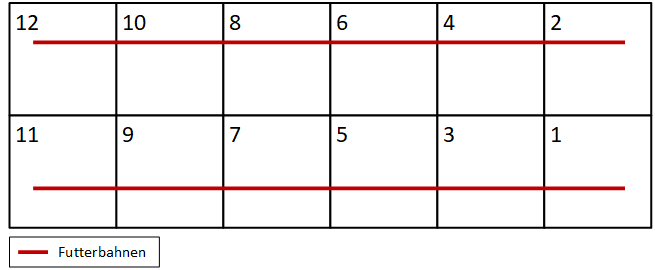
\includegraphics[width=0.9\textwidth]{img/Grafiken/Stallbereiche mit Futterbahn.png}
    \caption[Abteile des Mastputenstalls mit Verlauf der Futterbahnen.]{Abteile des Mastputenstalls mit Verlauf der Futterbahnen. Die Nummer in den oberen linken Ecken stehen für die IDs der Kameras.}
    \label{fig:KamerasImStall}
\end{figure}

Die Kameras nahmen einen Videostream auf. Die Bildinformationen wurden verwendet, um ein \gls{Detektion}[s]\glsdisp{Modul}{modul} anzuwenden. Dieses \glsdisp{Detektion}{detektierte} und \glsdisp{Lokalisation}{lokalisierte} die Puten im \gls{Frame}. Die \gls{Detektion} verlief in Echtzeit. Die \gls{Detektion}[en] wurde in einer Datenbank gespeichert, die sich auf einem Server befindet. Jeder Eintrag beinhaltet einen eindeutigen Zeitstempel und ein dazugehöriges \gls{Frame} in einem Videostream. Die Videostreams wurden auf Festplatten gespeichert. Insgesamt wurden  drei Mastdurchläufe aufgezeichnet. Ein Lebenszyklus der Puten umfasst ca. 4 Monate. Nach einer Aufzuchtphase von einem Monat kommen die Tiere in den Mastputenstall. Ab diesem Punkt begann die Datenerfassung. \par

Die Datensammlung im Mastputenstall war bereits vor Beginn dieser Arbeit abgeschlossen. Somit ließ sich kein Einfluss auf die Art und die Menge der zur Verfügung stehende Rohdaten nehmen. Die Videostreams liegen im mp4-Dateiformat vor. Das direkte Arbeiten auf der Datenbank mit den \gls{Detektion}[en] ist wegen des Datenvolumens und der Rechenleistung der Server nicht praktikabel. Aus diesem Grund wurde ein Tool entwickelt, das auf die Datenbank zugreift und Daten eines angegebenen Zeitintervalls herunterlädt. Die heruntergeladenen \gls{Detektion}[en] speichert das Tool in einer csv-Datei. In einer vorausgegangenen Arbeit im Rahmen des \acrshort{OptiLiMa} Projekts wurde ein \gls{Assoziation}[s]\glsdisp{Modul}{modul} entwickelt, das die \gls{Detektion}[en] nutzt. Somit steht ein \gls{MOT} System zur Verfügung. \par

Die \gls{Detektion} und die \gls{Assoziation} bauen auf dem Videostream auf. Jedes \gls{Frame} im Videostream hat einen eindeutigen Zeitstempel zugeordnet. Dadurch wird ersichtlich, dass die vorhandenen Rohdaten in Form von Zeitreihen vorliegen.

\subsection{Definition der Aufgabe} \label{sec:Meth DefAufgabe}
Ziel ist es, Verhaltensweisen der Mastputen zu klassifizieren (\autoref{sec:Zielsetzung}). Um eine Aufgabe zu formulieren, muss zunächst geklärt werden, was eine Verhaltensweise ist und wie sie sich erkennen lässt. In \cite{Levitis.2009} wird Tierverhalten definiert als Reaktionen von Individuen oder Gruppen auf Reize aus ihrer Umgebung. Das Suffix \textit{-weise} oder \textit{-art} bezeichnet eine Gewohnheit \cite{duden.art}. Eine Verhaltensweise ist somit ein Muster im Verhalten. Im Vorfeld dieser Arbeit wurden zwei Verhaltensweisen identifiziert, die besonders herausstechen. Diese werden hier als Kontrollgänge und Kämpfe bezeichnet. Im Folgenden werden diese beiden Verhaltensweisen erläutert. \dubpar

\begin{quote}

\textbf{Kontrollgänge}\par
Der Tierhalter unternimmt täglich Kontrollgänge im Maststall. Die Tiere reagieren auf den Tierhalter, wenn dieser den Stall betritt und umhergeht. Dabei finden Massenbewegungen statt. Die Tiere werden aufgeschreckt und fangen an, sich in Richtung des Tierhalters zu drängen. Oftmals beruhigen sich die Tiere noch während des Kontrollgangs. Nähert sich der Tierhalter ihrem Stallbereich, werden sie jedoch oftmals wieder aufgeschreckt und drängen sich erneut in seine Richtung. In seiner unmittelbaren Nähe weichen ihm die Tiere aus. Dadurch entsteht eine \gfuss{Traube} um den Tierhalter. Regelmäßig muss im Stall neues Stroh gestreut werden. Dafür fährt ein Traktor durch den Stall. Das Verhalten der Tiere ist in diesem Fall jedoch sehr ähnlich zum täglichen Kontrollgang. Die Tiere drängen zum Traktor. Um den Traktor bildet sich ein \gfuss{Traube}. Die \gfuss{Traube} ist dabei deutlich größer, aufgrund der Größe des Traktors. Fährt der Traktor durch den Stall, bleibt hinter ihm eine große freie Fläche zurück. Einige Puten nutzen diese Fläche, um dem Traktor nachzujagen. Teileweise füllt sich die Fläche jedoch nur gemächlich. Die Abbildung \ref{fig:bspKontrollg} zeigt einige Ausschnitte aus Kontrollgängen. 
\end{quote}


\begin{figure}[htb]
     \centering
     \begin{subfigure}[b]{0.4\textwidth}
         \centering
         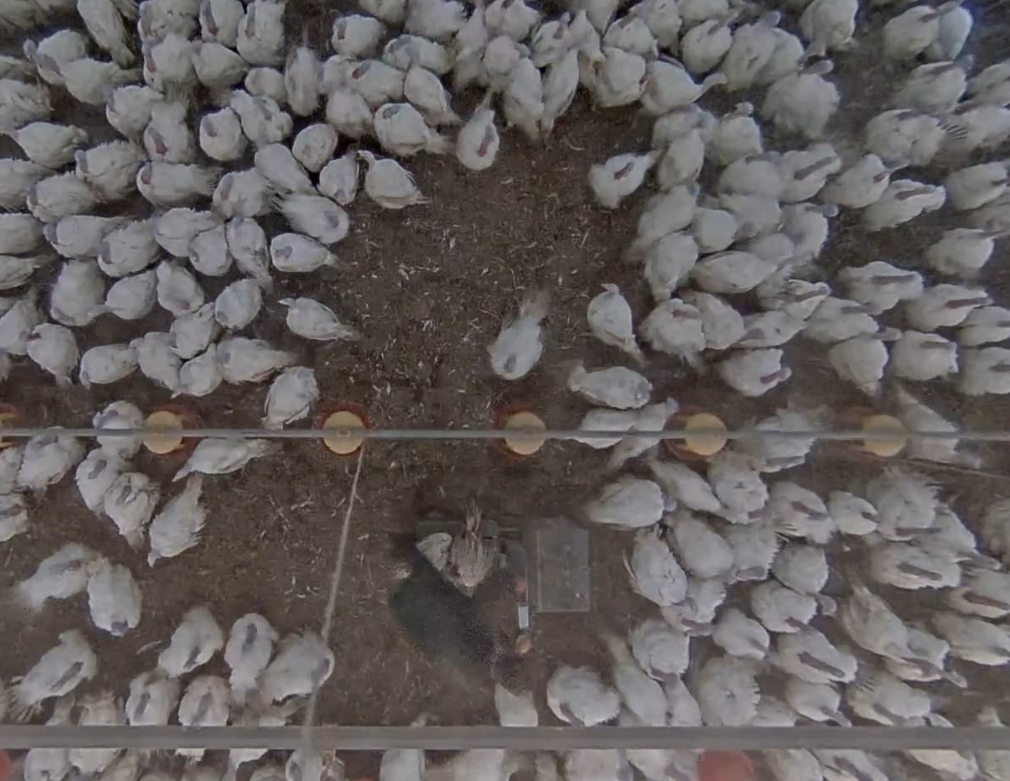
\includegraphics[width=\textwidth, height=5cm]{img/Verhaltensweisen/Kontrollgang Tierhalter Traube 2.png}
         \caption{Kontrollgang des Tierhalters.}
     \end{subfigure}
     \hfill
     \begin{subfigure}[b]{0.59\textwidth}
         \centering
         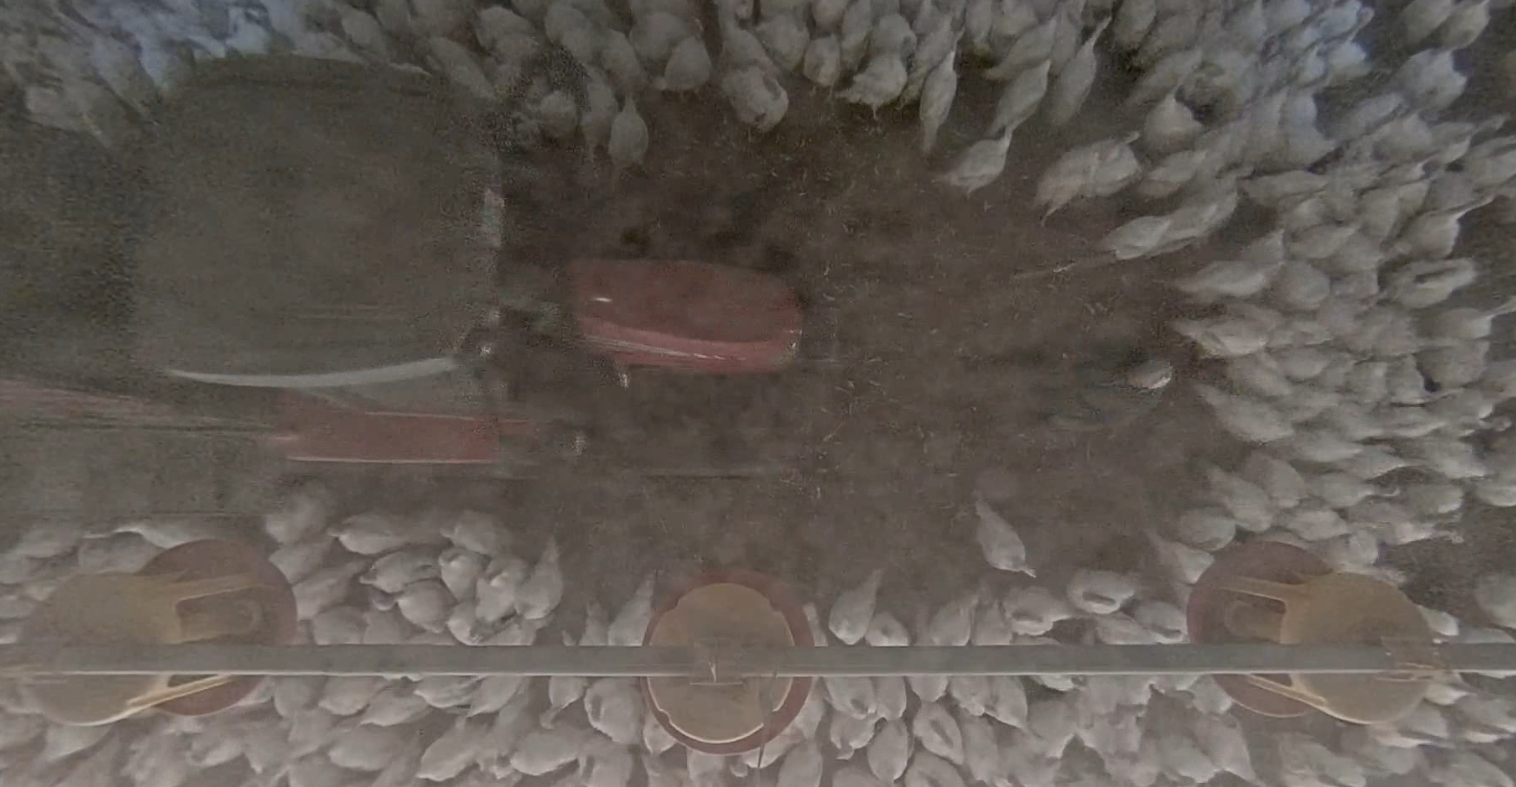
\includegraphics[width=\textwidth, height=5cm]{img/Verhaltensweisen/Kontrollgang Tracktor Traube.png}
         \caption{Einstreuung von Stroh mit Traktor.}
     \end{subfigure}
     \caption[Ausschnitte aus Kontrollgangereignissen.]{Ausschnitte aus Kontrollgangereignissen.}
     \label{fig:bspKontrollg}
\end{figure}


\par

\begin{quote}
\textbf{Kämpfe}\par
Ein Kampf entsteht ohne direkt ersichtlichen Auslöser. Ein Kampf beginnt meistens, indem sich zwei Tiere gegenüberstehen und sich gelegentlich versuchen anzupicken. Dies steigert sich meistens zu stärkeren Pickattacken. Dabei entwickeln die Tiere eine hohe Dynamik und bewegen sich umeinander. Oft passiert es, dass eine Pute die andere packt und um sich schleudert. Dadurch entstehen zirkulierende Bewegungsmuster. Die umliegenden Puten weichen den kämpfenden Tieren aus, wodurch eine \gfuss{Traube} entsteht. Auch Verfolgungen sind zu beobachten. Möchte eins der Tiere entkommen, jagt das andere diesem hinterher. Schafft es der Verfolger, die flüchtende Pute zu packen, wird der Kampf fortgesetzt. Die Verfolgungen finden mit hoher Dynamik statt. Es entstehen freie Flächen im Kanal der Fluchtbewegung. Ein Kampf muss nicht nur zwischen zwei Tieren stattfinden. Auch mehrerer Tiere können an einem Kampf beteiligt sein. Ebenfalls können die kämpfenden Tiere wechseln. Schafft es ein Tier zu flüchten und der Verfolger findet dieses nicht mehr, kann es sein, dass der Verfolger auf das nächstbeste Tier losgeht. Auch kann ein bisher unbeteiligtes Tier sich dazu entscheidet, in den Kampf mit einzusteigen. Der Kampf endet plötzlich und so, wie er begonnen hat, ohne ersichtlichen Auslöser. Die Abbildung \ref{fig:bspKämpf} zeigt einige Ausschnitte aus Kämpfen.
\end{quote}

\begin{figure}[htb]
     \centering
     \begin{subfigure}[b]{0.55\textwidth}
         \centering
         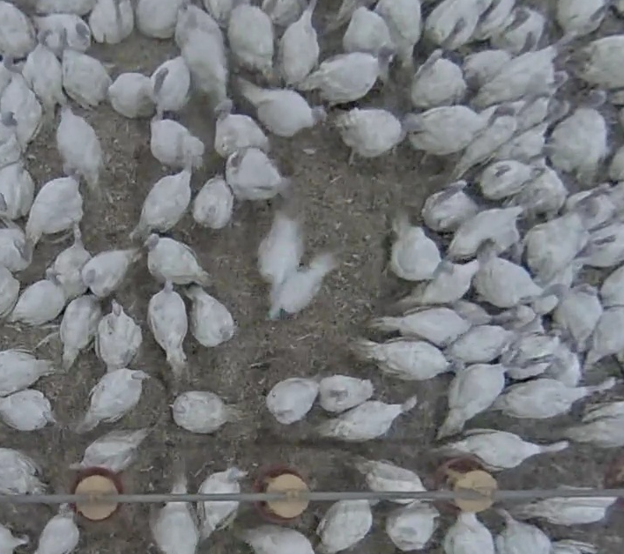
\includegraphics[width=\textwidth, height=6cm]{img/Verhaltensweisen/Kampf Traube.png}
         \caption{Kampf zwischen zwei Puten.}
     \end{subfigure}
     \hfill
     \begin{subfigure}[b]{0.44\textwidth}
         \centering
         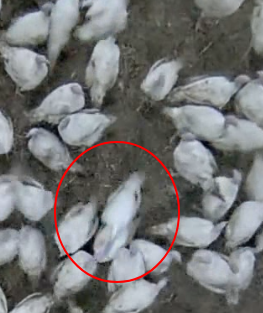
\includegraphics[width=\textwidth, height=6cm]{img/Verhaltensweisen/Kampf Verfolgung.png}
         \caption{Verfolgung eines flüchtenden Tieres.}
     \end{subfigure}
     \caption[Ausschnitte aus Kampfereignissen.]{Ausschnitte aus Kontrollgangereignissen.}
     \label{fig:bspKämpf}
\end{figure}

\par

Bei einem Kontrollgang treten dynamische Gruppenbewegungen auf, während Kämpfe durch dynamische Bewegungen vereinzelter Tiere geprägt sind. Bezogen auf den Kameraausschnitt ist bei einem Kontrollgang Dynamik in den meisten Bildbereichen zu beobachten. Kämpfe fallen durch lokale Dynamik in vereinzelten Bildbereichen auf. \par

Für diese Arbeit wurde jegliches Verhalten, was kein \textit{Kontrollgang} oder \textit{Kampf} ist, als \textit{Normalverhalten} deklariert. Der Begriff ist etwas irreführend gewählt, da \gfuss{Normalität} nicht näher definiert wurde. Jedoch sind Kämpfe und Kontrollgänge die auffälligsten Verhaltensweisen. Ebenfalls sind sie unerwünscht (\autoref{sec:Hintergrund}), weshalb der Fokus darauf gelegt wird, diese Verhaltensweisen vom restlichen Verhalten abzugrenzen. Das restliche Verhalten wird als \gfuss{Normal} bezeichnet. Die Definition der Merkmale von \textit{Normalverhalten} lässt sich aus diesem Grund als Abgrenzung von den anderen beiden Verhaltensweisen Formulieren.\dubpar

\begin{quote}
\textbf{Normalverhalten}\par
Während sich ein Kontrollgang durch eine globale hohe Dynamik auszeichnet und ein Kampf durch lokale hohe Dynamiken, so sind die Puten die meiste Zeit deutlich weniger aktiv. Bezogen auf die Bildbereiche der Kameras ruht sich ein Großteil der Tiere aus. Die Tiere sitzen stationär auf einer Position. Vermehrt tritt Aktivität rund um die Futterbahnen auf. Diese ist jedoch meistens nicht so dynamisch, wie in den anderen Verhaltensweisen.
\end{quote}
\par

Das Auftreten einer Verhaltensweise stellt für das geplante \gls{Modul} ein \gls{Ereignis} dar. Wie die Beschreibungen der Verhaltensweisen zeigen, basieren die charakterisierenden Merkmale vor allem auf der Bewegung der Tiere. Bewegung ist zeitabhängig. Die Merkmale der Verhaltensweise sind somit in einem Zeitraum zu beobachten. Ein \gls{Ereignis} wird also definiert durch einen Startzeitpunkt und einen Endzeitpunkt. Innerhalb dieser zeitlichen Grenzen sind die Merkmale der jeweiligen Verhaltensweise zu beobachten. \par

Aus den Anforderungen (\autoref{sec:Meth Anforderungen}) ist bekannt, dass ein \gls{Klassifikation}[sproblem] zu lösen ist. Durch die Erkenntnis, dass sich die \gls{Ereignis}[se] innerhalb eines Zeitraums abspielen und dem Fakt, dass auch die Rohdaten in Zeitreihen strukturiert sind (\autoref{sec:Meth RohDat}) wird deutlich, dass es sich bei der Aufgabe um eine \gls{Klassifikation} von Zeitreihen handelt.\par

\subsection{Aufbau des Gesamtkonzepts}
Die Aufgabe wurde definiert, die Rohdaten sind bekannt, das Format und die Merkmale der Verhaltensweisen wurden untersucht und die Modulanforderungen wurden formuliert. Mit diesem Wissen ist ein Gesamtkonzept für das \gls{Modul} zu entwicklen. Die Abbildung \ref{fig:GesKonzpt} zeigt dieses Konzept.

\begin{figure}[htb]
    \centering
    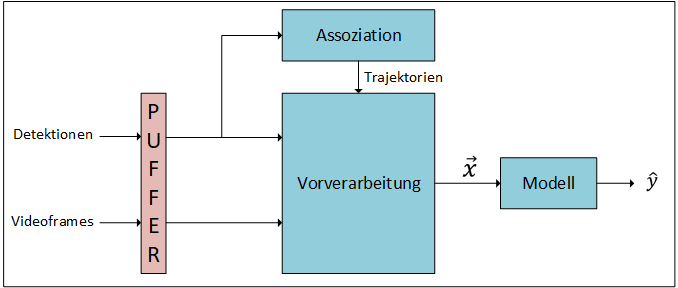
\includegraphics[width=0.9\textwidth]{img/Grafiken/Gesamtkonzept start.png}
    \caption{Gesamtkonzept des \gls{Modul}[s].}
    \label{fig:GesKonzpt}
\end{figure}


Ein Strom von Rohdaten fließt in das \gls{Modul}. Die \gls{Detektion}[sdaten] werden dem \gls{Assoziation}\glsdisp{Modul}{smodul} übergeben. Dieses generiert Trajektorien. Die Rohdaten und die Trajektorien fließen in einer Vorverarbeitung zusammen. Hier werden die \gls{Feature}[s] aus den Rohdaten extrahiert und konstruiert (\autoref{sec:ML FeatExtr}), die in der \gls{Feature}-Selektion (\autoref{sec:ML FeatSelect}) ausgewählt wurden. Nach der Vorverarbeitung wird der \gls{Featurevektor} dem ausgewählten (\autoref{sec:ML ModellSelect}), konfigurierten (\autoref{sec:ML HyperPara}) und trainierten (\autoref{sec:ML Metriken, Valid}) Modell übergeben. Das Modell schätzt, welche Verhaltensweise in der Probe zu beobachten ist und gibt ein \gls{Label} aus, das die Klassenzugehörigkeit eindeutig bestimmt. Dieses \gls{Label} ist auch die Ausgabe des \gls{Modul}[s]. \par

Da Zeitreihen \glsdisp{Klassifikation}{klassifiziert} werden müssen, ist die Vorverarbeitung der Rohdaten modellabhängig (\autoref{sec:sequenzen ML}). Nicht alle Modelle können Sequenzen direkt Verarbeiten. Wie \autoref{sec:Meth Nutzwert} zeigt, besitzen die vielversprechendsten Modelle kein Sequenzverständnis. Das Modell muss \gls{Feature}[s] erhalten, welche die Information der Zeitreihe komprimieren. Der Pufferspeicher ist dazu da, die einzelnen Zeitschritte der sequenziellen Rohdaten zu speichern. Sobald genügend Zeitschritte vorhanden sind, werden die Rohdaten an die Vorverarbeitung weitergegeben. Dort wird die gepufferte Sequenz zu einem einzelnen Datenpunkt komprimiert. 
\section{Bewertung des MOT-Systems}
Mit eine \gls{MOT} System sollen \gls{Trajektorie}[n] generiert werden um diese für \gls{Feature}[s] zu nutzen. In \ref{sec:Meth DefAufgabe} wird dargestellt, dass die Merkmale der Verhaltensweisen stark auf der Bewegung der Puten basieren. Über die \gls{Trajektorie}[n] sollen diese Informationen extrahiert werden können. Um das zu gewährleisten muss das \gls{MOT} System gut genug sein, um die Bewegungsmerkmale jeglicher Verhaltensweisen zu erfassen. Dies ist durch die Bewertung des \gls{MOT} Systems zu überprüfen. \par

Für die Evaluation des \gls{MOT} Systems ist eine \gls{Ground Truth} notwendig. Da die Evaluation Gültigkeit für einen sehr konkreten Anwendungsfall haben soll, ist es sinnvoll eine anwendungsbezogene \gls{Ground Truth} zu verwenden, anstatt Benchmarking Datensätze. \gls{Ground Truth}[s] für zwei Ereignisse wurden bereits vor dieser Arbeit erstellt. Wie in \ref{sec:MOT GT} dargestellt ist die Erstellung einer qualitativ hochwertigen \gls{Ground Truth} herausfordernd. Um die Aussagekraft der Evaluation beurteilen zu können, wird die Qualität der \gls{Ground Truth} diskutiert. \par

Für das \glsdisp{Assoziation}{Assoziationsmodul} ist ein Algorithmus auszuwählen. Zur Auswahl steht der \acrshort{SORT} Algorithmus (\ref{sec:MOT SORT}) und eine modifizierte Variante des Crocker-Grier Linking Algorithmus (\ref{sec:MOT CrockGrier}). Die Modifikationen werden in \ref{sec:Meth CrockGrieMods} erläutert. Für das Gesamtsystem ist zu Bewerten, welcher der Algorithmen die besten \gls{Feature}[s] gewährleisten kann. \par

Während der Versuche werden die Laufzeiten der Algorithmen gemessen, da diese relevant sind im Bezug auf die Echtzeitfähigkeit des Moduls. 


\subsection{Diskussion der Ground Truth Qualität} \label{sec:Meth GT Quali}
Noch vor dieser Arbeit sind zu zwei Ereignissen \gls{Ground Truth}[s] erstellt worden. Ein Kampfereignis und ein Kontrollgangereignis. Die Ereignisse sind jeweils eine Minute lang. Das Kampfereignis umfasst 91 \gls{Frame}[s], das Kontrollgangereignis umfasst 98 \gls{Frame}[s]. Dadurch ergiebt sich eine durchschnittliche \gls{Frame}[rate] von 1,6 \gls{Frame}[s] pro Sekunde. Die Ereignisse wurden von unterschiedlichen Personen bearbeitet.  \par

Die Herausforderungen, die die Erstellung einer qualitativ hochwertigen \gls{Ground Truth} mit sich bringt, waren zum Zeitpunkt der Erstellung nicht bewusst. Aus diesem Grund wurden keine klar definierten Regeln festgelegt, wie mit Mehrdeutigkeiten und anderen komplizieren Situationen umzugehen ist. Ganz ohne Regeln erfolgte die Erstellung jedoch nicht. Im Vorfeld wurde definiert, dass jedes Tier mit einer rechteckigen \gls{Bounding Box} zu \glsdisp{Detektion}{detektieren} ist. Die \gls{Bounding Box} soll das Tier möglichst eng, aber vollständig umschließen. Tiere sollen möglichst auch nach Verdeckungen korrekt \glsdisp{Assoziation}{assoziiert} werden. \par 

Bei der Überprüfung der \gls{Ground Truth} viel auf, die \gls{Detektion} funktionierte relativ zuversichtlich. Auch die \gls{Lokalisation} ist zufriedenstellend, auch wenn Schwankungen zu erwarten sind. Schwächen sind vor allem bei Mehrdeutigkeiten vorhanden. Die \gls{Detektion} bei teilweisen Verdeckungen ist inkonstant. Auch haben die unterschiedlichen Bearbeiter mehrdeutige Situationen unterschiedlich gelöst. Dadurch ist zu erwarten, dass Unsicherheiten in der Bewertung des \gls{Detektion}[smoduls] entstehen. Die Überprüfung zeigte, dass die \gls{Ground Truth} tendenziell eher Übermäßig optimistische Erwartungen an die \gls{Detektion} stellt. Bei teilweisen Verdeckungen wurde ein Tier länger \glsdisp{Detektion}{detektiert}, als es das \gls{Detektion}[smodul] tat. Somit ist mit einer vermehrten Anzahl von falsch negativen \gls{Detektion}[en] (\ref{sec:MOT Fehlertypen}) zu rechnen. \par

Die niedrige \gls{Frame}[rate], sowie die hohe Tierdichte im Stall, sorgten dafür das sich Tiere teilweise nur schwer auseinander halten ließen. Dadurch ist mit Unsicherheiten in der Evaluation des \gls{Assoziation}[smoduls] zu rechnen. 

Es ist empfehlenswert, dass das \gls{Detektion}[smodul] mit Daten trainiert wird, die aus der gleichen Quelle stammen wie die \gls{Ground Truth}. Das stellt eine faire Bewertung sicher, da keine diskrepanz vorhanden ist zwischen dem was das \gls{Detektion}[smodul] lernt und dem was die Evaluation von ihm fordert. Dies war hier nicht möglich, da die \gls{Detektion} bereits abgeschlossen war als die \gls{Ground Truth} erstellt wurde. Dadurch ist mit Unsicherheiten der Bewertung des \gls{Detektion}[smoduls] und des \gls{Lokalisation}[smoduls] zu rechnen.\par

Mit Fehlern in einer \gls{Ground Truth} ist zu rechnen. Um dennoch stabile Ergebnisse zu erhalten wird empfohlen mehrere \gls{Ground Truth}[s] zu verwenden und die Ergebnisse zu mitteln. Für die Bewertung bezogen auf den Anwendungsfall stehen jedoch nur zwei \gls{Ground Truth} Datensätze zur Verfügung. Das kann die Stabilität der Wertungen negativ beeinflussen.


\subsection{Modifikation des Crocker-Grier Linking Algorithmus} \label{sec:Meth CrockGrieMods}
Der grundlegende Aufbau des Crocker-Grier Linking Algorithmus ist in \ref{sec:MOT CrockGrier} erläutert. Die Modifikationen erfolgten bereits vor dieser Arbeit. Sie werden hier erläutert, um die Nachvollziehbarkeit der Arbeitsweise zu ermöglichen. \par

Bei der Anwendung der ursprünglichen Form des Crocker-Grier Linking Algorithmus auf Ereignisse im Putenmaststall, kam es zu Problemen. Die maximale Distanz \(l\) die ein Objekt zwischen zwei \gls{Frame}[s] zurücklegen darf, um korrekt \glsdisp{Assoziation}{assoziiert} werden zu können, wird von den Tieren oftmals nicht eingehalten. Gerade bei dynamischen Ereignissen legen die Puten in kürzerer Zeit, weitere Strecken zurück. Dies ist auch der niedrigen \gls{Frame}[rate] und hohen Tierdichte geschuldet. Durch die Verletzung von \(l\) entstehen \gls{Assoziation}[sfehler] (\ref{sec:MOT Fehlertypen}). Durch die Vergrößerung von \(l\) entstehen größere Netzwerke. In der Anwendung wurden die Netzwerke schnell so groß, dass die Rechenzeit unpraktikabel wurde.\par

Um diesen Problemen zu begegnen wurde eine iterative \gls{Assoziation} umgesetzt. Diese durchläuft mehrere Stufen, in denen die \gls{Assoziation} wiederholt wird. Bei jeder Iteration wird \(l\) vergrößert. Korrekte \gls{Assoziation}[en] werden in den folgenden Stufen nicht mehr betrachtet. Insgesamt werden drei Iterationen durchlaufen. Die Abbildung \ref{fig:funkCrockGrierMod} zeigt die Auswirkungen dieses Ansatzes. In der ersten Stufe werden vor allen stationäre Puten \glsdisp{Assoziation}{assoziiert}. Diese werden in den folgenden Stufen nicht mehr betrachtet. Dadurch wird der Abstand zwischen den zu \glsdisp{Assoziation}{assoziierenden} Objekten größer und korrekte \gls{Assoziation}[en] sind auch mit einem größeren \(l\) zu erwarten. Auch die Größen der entstehenden Netzwerke sind besser handhabbar. 

\emptyFigure{Stufen des Trackings, aus BA nehmen}{fig:funkCrockGrierMod}
\todo{Abbildung fehlt}

Gerade bei hoch dynamischen Ereignissen passiert es, dass in frühen Stufen nur wenige \gls{Assoziation}[en] getätigt werden können. Dadurch entstehen wieder mehr \gls{Assoziation}[sfehler]. Auch ist nicht mehr zu gewährleisten, dass der Rechenaufwand handhabbar bleibt. Aus diesem Grund wird in diesen Situationen das adaptive Verfahren angewendet, was in der \gls{Bibliothek} \textit{Trackpy} \cite{Allan.2023} implementiert ist. Dadurch wird sichergestellt, dass die Netzwerke eine Maximalgröße nicht überschreiten und der Rechenaufwand bleibt handhabbar. \par

Ziel ist es konstante \gls{Trajektorie}[n] zu generieren. Durch die Iterationen der Stufen können jedoch \gls{Fragmentation}[sfehler] provoziert werden. Das ist in der Abbildung \ref{fig:bspCrockGrierFrag} dargestellt. Unterbricht ein aktives Tier seine dynamische Bewegung für Wenige \gls{Frame}[s] und verweilt auf einer Position, dann werden die \gls{Assoziation}[en] dieser wenigen \gls{Frame}[s] bereits in einer früheren Stufe getätigt. Die \gls{Detektion}[en] der dynamischen Bewegung werden erst in höheren Stufen \glsdisp{Assoziation}{assoziiert}. Eine konstante \gls{Trajektorie} ist dann nicht mehr möglich, da das Verweilen des Tieres bereits aus der weiteren Betrachtung herausgenommen wurde. 

\emptyFigure{Fragmentation durch Stufen}{fig:bspCrockGrierFrag}
\todo{Abbildung fehlt}

Um solche Fehler zu vermeiden wurde ein Verifikatoinsmechanismus eingeführt, welcher evaluiert, ob eine \gls{Trajektorie} in einer bestimmten Stufe plausibel ist, oder nicht. ist die \gls{Trajektorie} plausibel, gilt sie als verifiziert und sie wird in das Ergebnis des \gls{MOT} Systems aufgenommen. Kann die \gls{Trajektorie} nicht verifiziert werden, dann kommen ihrer \gls{Detektion}[en] in die nächste Stufe. \gls{Detektion}[en], welche sich am Ende nicht in einer verifizierten \gls{Trajektorie} befinden, werden verworfen. Die Abbildung \ref{fig:TreeCrockGrierVerif} zeigt den Verifkationsmechanismus in Form eines Baumdiagramms. 

\emptyFigure{Verifikationsmechanismus}{fig:TreeCrockGrierVerif}
\todo{Abbildung fehlt}

Für die Verifikation wird das Video des Ereignisses mit herangezogen. Bei diesem wird ermittelt wie sich die Pixeln von \gls{Frame} zu \gls{Frame} verändern. Wenn \(\nommat{PIX}_t\) die Matrix aller Pixel in einem \gls{Frame} \(t\) ist, dann berechnet sich die Veränderung wie in \ref{eq:Pixelveränderung} dargestellt.

\begin{equation}
\text{Pixelveränderung} = \frac{abs(\nommat{PIX}_t - \nommat{PIX}_{t-1})}{\text{Pixelanzahl}}
\label{eq:Pixelveränderung}
\end{equation}

Dabei werden die Farbkanäle berücksichtigt. Ein \(Pixel \in \nommat{PIX}\) besitzt jeweils einen Kanal für rot, blau und grün. Diese können die Werte \(\{0,1,2, \dots, 255\}\) annehmen. Mathematisch lässt sich jeder Pixel als Vektor \(\nomvec{pix}\) betrachten. Der Wertebereich der Pixelveränderung somit \([0, 765]\), da \(3 \cdot 255 = 765\). \par

Der Verlauf der Pixelveränderung wird für das Ereignis ermittelt. Sie dient als Aktivitätsindikator. Eine \gls{Trajektorie} muss nicht über das gesamte Ereignis verlaufen. Es wird der Zeitraum betrachtet, in dem die \gls{Trajektorie} aktiv war. Für diesen Zeitraum wird die mittlere Pixelveränderung berechnet und die Standdardabweichung. Diese Werte dienen dazu um zu beurteilen, ob das Geschehen im Stall insgesamt Dynamisch ist, oder nicht. Bei einem dynamischen Geschehen, wie bei einem Kontrollgang, ist es sinnvoll die \gls{Detektion}[en] bei einem größeren \(l\) zu betrachten, da \gls{Fragmentation}[sfehler] wahrscheinlicher sind. \par

Die mittlere Geschwindigkeit aller \gls{Trajektorie}[n] wird berechnet und die Geschwindigkeit der individuellen \gls{Trajektorie}[n] wird damit verglichen. Liegt die Geschwindigkeit auffällig höher, als die mittlere Geschwindigkeit, wird das Potential für \gls{Fragmentation}[sfehler] als höher eingestuft und die \gls{Detektion}[en] werden in der nächsten Stufe erneut beurteilt. \par

Das letzte Verifikationskriterium ist die Schrittanzahl der \gls{Trajektorie}[n]. Von \gls{Trajektorie}[n], die über viele \gls{Frame}[s] verlaufen ist tendenziell zu erwarten, dass sie konstanter sind. Somit fordert der Verifikationsmechanismus eine minimale \gls{Frame}[anzahl], oder Anzahl von Zeitschritten.\par

Die Die Verifikationskriterien der unterschiedlichen Stufen sind dynamisch. Da in höheren Stufen eine höhere Fehleranfälligkeit erwartet wird, sinkt die minimale \gls{Frame}[anzahl], um nicht zu viele \gls{Trajektorie}[n] auszusortieren. Auch die Toleranzschranken für die Dynamik steigen, da in den höheren Stufen mehr Dynamik erwartet wird. \par



\subsection{Methodisches Vorgehen der MOT Evaluationen}
Für die Evaluation stehen zwei \gls{Ground Truth} Ereignisse zur Verfügung. Ein Kampfereignis und ein Kontrollgangereignis (\ref{sec:Meth GT Quali}). Die Algorithmen, zwischen denen Auszuwählen ist sind der \acrshort{SORT} Algorithmus (\ref{sec:MOT SORT}) und die modifizierte Variante des Crocker-Grier Linking Algorithmus (\ref{sec:Meth CrockGrieMods}). Die Evaluation wird mittels der \gls{HOTA} Metrik (\ref{sec:MOT HOTA}) durchgeführt, da mit dieser Metrik die fairste Bewertung zu erwarten ist und die genausten Fehleranalysen. Die \textit{\gls{IDF1}-Metrik} und die \textit{\acrshort{CLEAR} \gls{MOT}} Metriken werden jedoch angegeben, da sie etablierter sind als \gls{HOTA}. Für die Berechnung der Metriken wird die Software \textit{TrackEval} benutzt \cite{TrackEval.2020}. Diese ist die offizielle Evaluationsoftware der \textit{MOTChallenge} und steht als Open-Source Code zur Verfügung. Mit der Nutzung von \textit{TrackEval} wird sichergestellt, dass die Metriken korrekt berechnet werden. \par

Als erstes wird für beide Algorithmen die Gesamtperformance bewertet. Dazu werden die beiden Algorithmen auf die Ereignisse angewendet zu denen \gls{Ground Truth}[s] vorhanden sind. Für jeden \gls{Assoziation}[salgorithmus] ist anschließend ein Trackingergebnis vorhanden. Dieses beinhaltet die \gls{Trajektorie}[n]. Gespeichert werden die Trackingergebnisse als txt-Datei. Die Formatierung erfolgt angepasst an \textit{TrackEval}, gemäß \cite{MOT15}. Anschließend werden die Metriken berechnet. Wie \textit{TrackEval} auf eigene \gls{MOT} Systeme und mit eigenen \gls{Ground Truth}[s] anzuwenden ist, ist in der Dokumentation erläutert \cite{TrackEval.2020}. Die Evaluation der beiden Ereignisse wird gemittelt. Die Ergebnisse der beiden Algorithmen lassen sich vergleichen. Neben den Wertungen der \gls{HOTA} Metrik, erstellt \textit{TrackEval} einen Plot. Dieser zeigt den Verlauf der Wertungen über \(\alpha\). Die Abbildung \ref{fig:MPNTrack} zeigt einen solchen Plot. Dieser ist einem \gls{MOT} System namens \textit{MPNTrack} entnommen, welcher bei der \textit{MOTChallenge} 2016 und 2017 angetreten ist. Dieser ist hier zu Beispielzwecken angeführt. 

\emptyFigure{MPNTrack MOT17 bsp}{fig:MPNTrack}
\todo{Abbildung fehlt}

Während der Generation der Trajektorien werden die Laufzeiten der Algorithmen gemessen. Ebenfalls werden weitere Laufzeitmessungen durchgeführt, bei denen die Länge der Ereignisse stärker zu variieren sind. Dadurch ist ein Vergleich der Laufzeiten möglich und auch wie die Laufzeiten im Bezug auf die Ereignisslänge Skalieren.\par 

Als nächstes ist zu überprüfen, ob die \gls{Assoziation}[salgorithmen] alle Verhaltensweisen 
gleich gut \glsdisp{Assoziation}{assoziiert} bekommen. Dazu wird jedes Ereignis unabhängig von einander evaluiert.\par

\section{Nutzwertanalyse zur Vorauswahl von Machine Learning Modellen} \label{sec:Meth Nutzwert}
Für das \gls{Modul} zur Verhaltensklassifizierung wird ein Algorithmus des \glsdisp{ML}{maschinellen Lernens} benötigt. Die Auswahl eines passenden Algorithmus ist oftmals nur durch ausprobieren verschiedener Algorithmen möglich. Um Zeit einzusparen ist es Sinnvoll die Auswahl einzugrenzen \ref{sec:ML ModellSelect}. Diese Eingrenzung wird hier mittels einer Nutzwertanalyse durchgeführt. \par

Eine Nutzwertanalyse ist eine Methode zur Entscheidungsfindung, bei welcher Entscheidungsalternativen mittels einer Wertung verglichen werden \cite{Kuhnapfel.2021}. Sie ist jedoch anfällig für eine subjektive Bewertung der Entscheidungsalternativen. Aus diesem Grund wird sie hier nur für eine Eingrenzung der Auswahl verwendet und nicht für eine finale Entscheidung. Bei einer Nutzwertanalyse werden Kriterien ausgewählt, anhand derer die Alternativen bewertet werden. Diese Kriterien erhalten eine Gewichtung, welche ihre Wichtigkeit verdeutlicht. Die Gewichte werden in Prozent angegeben und ergeben kumuliert 100 \%. Für eine Alternative wird der Erfüllungsgrad in Bezug auf ein Kriterium angegeben. Für diesen Erfüllungsgrad ist eine Skala notwendig, bspw. \(\{1,2,\dots,10\}\). Diese Skala wird für alle Kriterien verwendet. Der Grad der Erfüllung wird für jede Alternative in Bezug auf alle Kriterien angegeben und Gewichtet. Die Summe der gewichteten Erfüllungswerte einer Alternative sind der Nutzwert dieser Alternative. Die Abbildung \ref{fig:bspNutzwertanalyse} zeigt beispielhaft eine Nutzwertanalyse.

\emptyFigure{Nutzwertanalyse BSP}{fig:bspNutzwertanalyse}
\todo{Abbildung fehlt}


\subsection{Auswahl der Kriterien}
Zunächst werden die Kriterien vorgestellt mit denen die Nutzwertanalyse durchgeführt werden soll. Diese sind Ausgewählt in Bezug auf die Aufgabe und die Rahmenbedingungen. Als Bewertungsskala werden die Werte \(\{1,2,\dots,10\}\) verwendet. Wie die Skala an die Kriterien angesetzt wird, wird erläutert. Ebenfalls erfolgt eine Einschätzung der Wichtigkeit.\par

\textbf{Rechenaufwand:}\\
Die Anforderungen an die Rechenleistung der Algorithmen können sehr unterschiedlich sein. Rechenleistung 
steht jedoch nur begrenzt zur Verfügung. Es stehen zwei baugleiche Rechner zur Verfügung. Die Prozessoren 
habe 16 Kerne und sie haben eine maximale Taktfrequenz von 5.10 GHz. Als Grafikkarte steht nur die der 
Hauptplatine zur Verfügung. Bezogen auf die Skala bedeuten höhere Werte eine geringere Anforderung an die Rechenleistung. Das Kriterium ist als wichtig einzustufen.\par

\textbf{Datenmenge:}\\
Gerade komplexe Modelle wie im \gls{Deep Learning} benötigen eine große Datenmenge. Wie in \ref{sec:Meth Datensatz} genauer beschrieben wird, ist die Datenmenge relativ klein. Dadurch entsteht gefahr für \gls{Overfitting}, gerade bei komplexen Modellen. Bezogen auf die Skala bedeuten höhere Werte eine geringere Anforderung an die Datenmenge. Die Datenmenge hat einen sehr großen Einfluss und das Kriterium ist als sehr wichtig einzustufen. \par

\textbf{Sequenzverständins:}\\
Bei der Aufgabe handelt es sich um ein \gls{Klassifikation}[sproblem] von Zeitreihen (\ref{sec:Meth DefAufgabe}). Gutes Sequenzverständnis wäre eine nützliche Fährigkeit des Modells (\ref{sec:sequenzen ML}). Höhere Werte auf der Skala bedeuten ein besseres Sequenzverständnis. Die Fähigkeit ist sehr relevant für die Aufgabe, jedoch bestehen Möglichkeiten Sequenzen auch mit einfacheren Modellen zu verarbeiten. Aus diesem Grund ist das Kriterium nicht Entscheidend und als mittelmäßig wichtig zu gewichten. \par

\textbf{Komplexität des Anwendens:}\\
Komplexere Modelle sind i.d.R. auch komplexer Anzuwenden. Da in Bezug auf diese Arbeit, wenig Vorerfahrung mit \glsdisp{ML}{machniellem Lernen} vorhanden ist und der Zeitrahmen begrenzt ist, ist eine einfache Anwendbarkeit des Modells Vorteilhaft. Eine niedrige Komplexität erzielt auf der Skala einen höheren Wert. Aus den Zeit und Erfahrungsgründen ist das Kriterium relevant, jedoch ist das Ziel ein möglichst gutes Modell zu erhalten. Deshalb sollte das Kriterium nicht Entscheidungsgebend sein. Es wird als geringfügig wichtig gewichtet. \par

\textbf{Modellierfähigkeit:}\\
Modelle des \gls{Deep Learning} haben eine sehr hohe Modellierfähigkeit, während eine lineare Regression nur wenig komplexe Zusammenhänge modellieren kann. Es ist jedoch einfacher ein komplexeres Modell durch Regularisierung in seiner Modellierfähigkeit zu beschneiden, als ein zu einfaches Modell zu verwenden. Deshalb wird eine hohe Modellierfähigkeit mit hohen Werten der Skala bewertet. Eine sehr hohe Modellierfähigkeit sehr hoch zu Bewerten, kann sich verzerrend auf die Nutzewertanalyse auswirken. Eine sehr hohe Modellierfähigkeit kann zu \gls{Overfitting} führen, wenn die Rahmenbedingungen nicht Stimmen, wir z.B. eine ausreichende. Datenmenge. Um solchen Verzerrungen entgegen zu wirken, wird das Kriterium als geringfügig wichtig eingestuft. \par

\textbf{Geschwindigkeit der Schätzung:}\\
Da das \gls{Modul} für die Verhaltensklassifikation Echtzeitfähigkeit besitzen soll, ist die Geschwindigkeit der Ergebnisfindung des Modells wichtig. Eine hohe Geschwindigkeit erzielt hohe Wertungen auf der Skala. Die Geschwindigkeit der Schätzung ist sehr relevant für das Gesamtkonzept. Jedoch ist der Anwendungsfall nicht kritisch, weshalb keine harten Toleranzgrenzen für die Echtzeitbedingung gelten. Die Wichtigkeit ist deshalb als geringfügig wichtig eingestuft. \par

In der Tabelle \ref{tab:NWAKriterien} ist eine Übersicht der Kriterien zu sehen. Die Wichtigkeit wurde versucht zu quantisieren. Ebenfalls ist Dargestellt wie die Skalen verlaufen.


\begin{table}[ht]
    \centering
    \begin{tabular}{|l|r|r|}
         \hline
         \textbf{Kriterium}                      & \textbf{Skala \(\{1,2,\dots,10\}\)}    & \textbf{Gewichtung}\\
         \hline
         Rechenaufwand                  & hoch \dots niedrig            & 25 \%\\
         \hline
         Datenmenge                     & hoch \dots niedrig            & 34 \%\\
         \hline
         Sequenzverständnis             & niedrig \dots hoch            & 17 \%\\
         \hline
         Komplexität des Anwendens      & hoch \dots niedrig            & 8 \%\\
         \hline
         Modellierfähigkeit             & niedrig \dots hoch            & 8 \%\\
         \hline
         Schätzungsgeschwindigkeit  & niedrig \dots hoch            & 8 \%\\
         \hline
         \textbf{Summe}                 &                               & 100 \%\\
         \hline
    \end{tabular}
    \caption{Übersicht über die Kriterien für die Nutzwertanalyse und ihre Gewichte.}
    \label{tab:NWAKriterien}
\end{table}

\subsection{Abwägung der Algorithmen}
Die Algorithmen zwischen denen abgewägt werden soll, sind in \ref{sec:ML Algorithmen} vorgestellt. Sie werden hier im Bezug auf die Kriterien diskutiert. Abschließend wird die Nutzwertanalyse präsentiert und die Auswahl der Algorithmen eingegrenzt. \par

\textbf{k-Means Algorithmus}\\
Der k-Means Algorithmus besitzt kein direktes Sequenzverständnis. Doch es bietet sich an Distanzmetriken für Zeitreihen einzusetzen, um eine Clusteranalyse anhand der Ähnlichkeit der zeitreihen durchzuführen. Auch die Option komprimierte \gls{Feature}[s] zu verwenden ist gegeben. Der Algorithmus ist an für sich nicht besonders Anspruchsvoll in seinem Rechenaufwand. In Kombination mit Distanzmetriken für Sequenzen, können diese dafür sorgen, dass der Aufwand steigt. Die Berechnung von solchen Distanzmetriken, wie Dynamik Time Warping kann Rechenaufwändig sein. Eine k-Means Clusteranalyse ist bereits mit einer relativ kleinen Datenmenge gut durchführbar. Die Anwendung ist prinzipiell sehr einfach, da meistens nur ein einziger \gls{Hyperparameter}, die Clusteranzahl benötigt wird. Jedoch liegt auch genau hier die Schwierigkeit. Die Clusteranzahl muss im Vorhinein bestimmt werden. Diese zu Ermitteln kann aufwendig sein. Implementationen des Algorithmus sind in verschiedenen Software-\gls{Bibliothek}[en] zu finden \cite{FabianPedregosa.2011}. Die Modellierfähigkeit ist begrenzt aus mehreren Gründen. Zum einen lernt das Modell unüberwacht, wodurch der Lernprozess nicht kontrollierbar ist. Das sorgt dafür, dass auch die Modellierung nur schwierig anzupassen ist. Zusätzlich ist das Vorgehen wenig komplex, wodurch wichtige Zusammenhänge in den \gls{Feature}[s] eventuell nicht gefunden werden. Von der Geschwindigkeit der Schätzung ist nicht davon auszugehen, dass sie problematisch seien wird.

\textbf{Hierarchisches Clustering}
Das hierarchische Clustering ist in den meisten Aspekten ähnlich einzustufen wie der k-Means Algorithmus. Der Hauptunterschied liegt darin, dass die Cluster selbst gefunden werden, ohne vorweg eingestellt werden zu müssen. Das macht die Anwendung einfacher als beim k-Means Algorithmus.\par

\textbf{Logistische Regression}
Die Logistische Regression ist, wie in \ref{sec:ML Algorithmen} dargestellt im Grunde ein lineares Modell. Das macht die Berechnung relativ einfach. Der Rechenaufwand ist dem entsprechend nicht sonderlich hoch. Jedoch ist das Modell dadurch auch nicht besonders komplex, was die Modellierfähigkeit begrenzt. Da es jedoch überwacht lernt und Regularisierung möglich ist, ist es deutlich Anpassbarer als k-Means und das hierarchische Clustering. Es ist in der Lage mit einer relativ kleinen Datenmenge auszukommen und Das Modell ist einfach anzuwenden. Auch die Dauer der Schätzung ist sehr gering zu erwarten, da die Berechnung des Ergebnisses im Kern mittels einer linearen Gleichung erfolgt. Reihenfolgen in Daten kann das Modell nicht berücksichtigen. Sequenzverständnis ist deshalb nur mit der Komprimierung der Zeitreihen möglich.\par

\textbf{Support Vector Machines}
\acrshort{SVM}[s] basieren im Kern auch auf einem linearen Modell, wodurch sie im Bezug auf den Rechenaufwand, die Datenmenge der Komplexität des Anwendens und der Schätzungsgeschwindigkeit ähnlich sind wie die logistische Regression. Da \acrshort{SVM}[s] jedoch durch Modifikationen auch in der Lage sind nicht-lineare Modelle zu erstellen ist die Modellierfähigkeit besser als bei der logistischen Regression. Dies kann jedoch den Rechenaufwand erhöhen.\par

\textbf{Random Forest}
Da das Random Forest Modell seine Entscheidungsbäume parallel erstellt, lässt es sich mit mehreren Prozessorkernen effizient erstellen. Da es jedoch mehrere einfache Modelle verwendet, ist der Rechenaufwand dennoch höher als bei der \acrshort{SVM} oder der linearen Regression. Dafür ist Modellierfähigkeit besser. Zu Konfigurtation des Modells sind mehr Hyperparameter einstellbar. Das macht die Anwednung etwas komplexer, als bei der SVM und der linearen Regression. In der Regel benötigt das Modell etwas mehr Daten als die linearen Modelle, jedoch ist die Modellkomplexität durch die Hyperparameter gut einstellbar, so dass eine geringe Datenmenge ausreichen kann. Die Schätzgeschwindigkeit ist höher zu erwarten als bei den linearen Modellen, da die Ergebnisfindung aus zwei Schritten besteht. Im ersten finden die einzelnen Bäume eine Lösung und im Zweiten wird die Mehrheit ermittelt. Das Sequenzverständnis ist genau so gut wie bei den linearen Modellen.\par

\textbf{Gradient Boosting}
Gradient Boosting ist Rechenintensiver als Random Forest. Durch die sequentielle Erstellung der Bäume ist das Training nicht parallelisierbar. In der Regel ist das Modell Modellierfähiger als Random Forest. Durch das erlernen wie es Fehler korrigieren muss, wird das Modell besser auf die Daten zugeschnitten, jedoch ist das Potenzial für Overfitting dadurch höher als bei Random Forest. In den anderen Kriterien ist eine ähnlich gute Performance zu erwarten wie bei Random Forest.\par

\textbf{Long Short Term Memory}
Der große Vorteil von LSTMs und Deep Learning für die Aufgabe ist, dass sie Sequenzen verstehen können. Dadurch muss nicht mit Informationsverlust durch Komprimierung gerechnet werden. Deep Learning Modelle sind extrem Modellierfähig, jedoch auch komplex anzuwenden, da sie viele Hyperparameter besitzen. Für einfachere Aufgaben sind jedoch auch Netzwerke möglich, die nur wenige Schichten haben, wodurch die Komplexität überschaubar bleibt. Dadurch das mehrere Schichten durchlaufen werden, ist mit einer erhöhten Dauer für die Ergebnisfindung zu rechnen. Deep Learning benötigt jede Menge Daten und viel Rechenleistung. 

\textbf{Gated Recurrent Unit}
Die GRU ist in den meisten Kriterien ähnlich zu bewerten wie das LSTM, aus den gleichen Gründen. Durch die reduzierte Komplexität der GRU ist mit einem etwas geringeren Rechenaufwand auszugehen. Auch die benötigte Datenmenge ist dadurch vermutlich etwas geringer.\ar

\begin{table}[ht]
\centering
\setlength{\tabcolsep}{11pt}
\caption{Nutzwertanalyse der Modelle}
\begin{tabular}{
    l
    S[table-format = 1.2]
    *{6}{S[table-format=2.0]} % Formatierung für die Zahlen ohne Dezimalstellen
    S[table-format=2.2]
    S[table-format=1.0]
  }
\toprule
Kriterien & 
\rotatebox{90}{Gewicht} & 
\rotatebox{90}{k-Means} & 
\rotatebox{90}{Hierarchisches Clustering} & 
\rotatebox{90}{Logistische Regression} & 
\rotatebox{90}{SVM} & 
\rotatebox{90}{Random Forest} & 
\rotatebox{90}{Gradient Boosting} & 
\rotatebox{90}{LSTM} & 
\rotatebox{90}{GRU}  \\
\midrule
Rechenaufwand               & 0,25 & 6 & 6 & 10 & 9  & 8 & 7 & 1  & 2 \\
Datenmenge                  & 0,34 & 9 & 9 & 9  & 9  & 8 & 8 & 1  & 2 \\
Sequenzverständnis          & 0,17 & 5 & 5 & 4  & 4  & 4 & 4 & 10 & 10 \\
Komplexität des Anwendens   & 0,08 & 5 & 7 & 7  & 7  & 6 & 6 & 2  & 2 \\
Modellierfähigkeit          & 0,08 & 1 & 1 & 5  & 6  & 7 & 8 & 10 & 10 \\
Schätzungsgeschwindigkeit   & 0,08 & 9 & 9 & 10 & 10 & 8 & 8 & 5  & 5 \\
\midrule
\addlinespace % Extra Abstand vor der letzten Zeile
Nutzwert & {--} & 6,6 & 6,8 & 8,0 & 7,8 & 7,1 & 6,9 & 3,7 & 4,2 \\
Rang & {--} & 6 & 5 & 1 & 2 & 3 & 4 & 8 & 7 \\
\bottomrule
\end{tabular}
\end{table}


\input{chapters/methodenentwicklung/Entwicklung eines Konzepts für die Verifizierung und das Labeling der Ereignisse}
\section{Zusammensetzung des Ursprungsdatensatzes}
\section{Konzept zur Feature-Extraktion}
\section{Anwendung der Methoden des Feature-Engineerings}
Über das Konzept in \autoref{sec:Meth FeatExtr} können Features aus den Rohdaten extrahiert werden. Im Vorfeld ist die Frage zu beantworten, welche Features extrahiert werden sollen. Diese Features werden in \autoref{sec:Meth ExtrFeaturesVors} vorgestellt. Mit den extrahierten Features als Grundlagen lassen sich weitere Features konstruieren (\autoref{sec:ML FeatExtr}). Welche Methoden zur Feature-Konstruktion verwendet werden, wird in \autoref{sec:Meth KonstrFeatures} erläutert.


\subsection{Vorstellung der extrahierten Features} \label{sec:Meth ExtrFeaturesVors}
Die charakteristischen Merkmale der Verhaltensweisen sind in \autoref{sec:Meth DefAufgabe} dargestellt. Diese waren teilweise bereits bekannt und teilweise sind sie erst während der Verifizierung aufgefallen. Dadurch ist Fachwissen vorhanden, um maßgeschneiderte Features zu entwerfen. Fachwissen ist ein großer Vorteil für den Entwurf von Features, wie in \autoref{sec:ML FeatExtr} erläutert. Es ist sinnvoll, Bias einzuführen in Bezug auf die charakteristischen Merkmale. Features können so konstruiert werden, dass sie darauf ausgelegt sind, bestimmte Aspekte der charakteristischen Merkmale zu erfassen. Ebenfalls ist durch das Fachwissen und das Wissen, dass die Zusammensetzung der Ereignisse Bias-behaftet ist (\autoref{sec:Meth Datensatz}), besser abzuwägen, ob bestimmte Features den vorhandenen Bias verstärken. Auch können Features entworfen werden, die gezielt versuchen, den Bias abzuschwächen. \par

Das soll an einem Beispiel verdeutlicht werden. Ein charakteristisches Merkmal von Kontrollgängen sind prägnante Gruppenbewegungen. Die Tiere drängen kollektiv in Richtung des Tierhalters. Somit kann der Drift der Bewegung aller Tiere ein interessantes Feature sein. Die Driftrichtung würde jedoch den Bias in den Daten verstärken, da diese vermutlich sehr abhängig vom Stallbereich ist. Da die Ereignisse jedoch nur aus zwei Stallbereichen stammen, ist dies ein Feature, das die Generalisierung hinsichtlich aller Stallbereiche beeinträchtigen würde. Ein besseres Feature wäre der Betrag der Driftgeschwindigkeit. Dieser ist ein Indikator für eine starke kollektive Bewegung in eine unbestimmte Richtung und damit unabhängiger vom Stallbereich. \par 

Für die Feature-Erstellung ist nochmal darauf hinzuweisen, dass die Merkmale einer Sequenz, also eines Ereignisses, zu einem einzelnen Datenpunkt komprimiert werden. Die Features benutzen immer einen einzigen Wert, um eine Information aus mehreren Zeitschritten zusammenzufassen. Ebenfalls sind möglichst numerische Features zu erstellen, da gerade einfachere Modelle mit diesen besser umgehen können als mit kategorischen Features. Im Anhang findet sich eine Tabelle mit ausführlichen Beschreibungen der Features, die mit dem Konzept aus \autoref{sec:Meth FeatExtr} für den Trainingsdatensatz extrahiert werden. Insgesamt sind dies 40 Features. Diese werden im weiteren Verlauf Basis-Features genannt, da die weiteren Features aus diesen konstruiert werden.\par


\subsection{Konstruktion der Features} \label{sec:Meth KonstrFeatures}
Da eine ausführliche Analyse und Auswahl der Features geplant sind, wird bei der Konstruktion der Fokus auf Masse gelegt. Features werden mittels aller Konstruktionsmethoden generiert, die in \autoref{sec:ML FeatExtr} vorgestellt sind. Bei der Durchführung ist festzustellen, dass einige der Basis-Features keine Information beinhalten. Die minimale Entfernung und Kurvigkeit sind in allen Ereignissen konstant null. Diese werden aus der Feature-Menge entfernt, somit reduziert sich die Anzahl der Basis-Features auf 38.\par

Zunächst werden Interaktionsfeatures erschaffen, indem die Features paarweise multipliziert werden, um ein neues Feature zu generieren. Auch die Multiplikation mit sich selbst ist darin eingeschlossen. Es entstehen 741 neue Features, wodurch die Featureanzahl auf 779 steigt. Mittels Gruppierung werden die 779 Features in Perzentile eingeteilt und als Perzentil-Features bezeichnet. Ebenfalls werden die Power-Transformationen auf die 779 Features angewendet. Die logarithmische Transformation wird mit der Basis 10 durchgeführt, da sie vor allem die Größenordnungen stauchen soll. Auch die Box-Cox-Transformation für alle 779 Features eingesetzt. \par

Bei der Berechnung der Perzentil-Features ist die normierte maximale Schrittanzahl nicht gruppierbar, auch nicht in der Interaktion mit sich selbst. Das liegt an Invarianz in der Verteilung, da der Wert meistens 1 beträgt. Deshalb fallen diese beiden Features heraus. Neun weitere Features lassen sich aufgrund geringer Varianz zwar nicht in Perzentile, dafür aber in Dezile einteilen. Da die Bezeichnung Perzentil-Features somit faktisch nicht mehr korrekt ist, werden sie als Quantil-Features bezeichnet. \par

Ziel der Gruppierungen und Power-Transformationen ist es, jegliche Features, die Informationen beinhalten können, unterschiedlich zu skalieren und zu formatieren. In der Feature-Auswahl soll untersucht werden, welche Methode die Informationen des jeweiligen Features am besten verpackt. Die Tabelle \ref{tab:FeatureMenge} zeigt die Feature-Mengen nach der Transformation.


\begin{table}[ht]
    \centering
    \caption{Übersicht über die Feature-Mengen pro Kategorie.}
    \begin{tabular}{|l|r|}
        \hline
        Feature-Kategorie & Anzahl\\
        \hline
        Basis & 38 \\
        Interaktion & 741\\
        Quantile & 777\\
        Logarithmisch & 779\\
        Box-Cox & 779\\
        \hline
        \hline
        Gesamt & 3114\\
        \hline
    \end{tabular}
    \label{tab:FeatureMenge}
\end{table}
\section{Methoden zur Feature-Auswahl, Hyperparametersuche und Modellauswahl} \label{sec:Meth FeatHypModSelect}
zwischen der Feature-Auswahl, dem Modellauswahl und der Hyperparamtersuche besteht ein enger Zusammenhang. Werden für die Feature-Auswahl modellabhängige Methoden verwendet, wie die Wrapper Methoden, muss ein Modell vorhanden sein, mit welchem sich die Methoden anwenden lassen. Um zwischen unterschiedlichen Modellen auszuwählen auf Basis ihrer Performance, ist eine Einstellung der Hyperparameter notwendig, damit die Modell auch fair bewertet werden. Ein Modell \(A\) wird beispielsweise mit einem Modell \(B\) verglichen. Die Hyperparameter sind noch nicht eingestellt. Modell \(A\) erzielt eine bessere Performance. Anschließend werden passende Hyperparameter gesucht. Anschließend zeigt ein weiterer Vergleich, dass nun Modell \(B\) die bessere Wahl ist. \par

Um also ein möglichst effektives Modell zu erhalten, ist eine Grobe Voreinstellung der Hyperparameter durchzuführen der Modelle durchzuführen. Anschließend wird eine Methode für die Feature-Auswahl angewendet. Da die Modelle vorhanden und eingestellt sind, darf diese modellabhängig, oder modellunabhängig sein. Anschließend kann die Performance der Modelle verglichen werden. Das beste wird ausgewählt und eine Feineinstellung der Hyperparameter wird durchgeführt. Das finale wird mit dem Testdatensatz überprüft und kann anschließend angewendet werden.\par

Da die Hyperparametersuche über die Optimierung des Validierungsergebnisses geschieht und dafür Modelle trainiert werden müssen, benötigt es hier bereits gute Features. Aus diesem Grund wird eine Vorauswahl der Features durchgeführt, um die Menge der Features einzugrenzen. Da uninformative Features Underfitting verursachen können und redundante Features Overfitting provozieren können, ist ein Vorauswahl sinnvoll, um eine aussagekräftige Einschätzung der Generalisierfähigkeit der Modelle zu erhalten. \par

Da die Datenmenge sehr begrenzt ist, wie in \ref{sec:Meth Datensatz} dargestellt, wird für die Validierung Cross-Validation angewendet (\ref{sec:ML Metriken, Valid}). Für das Training und das Testen wird der Datensatz aus \ref{tab:DataNachBalance} in ein Trainingsdatensatz und einen Testdatensatz aufgeteilt. 20 \% der Datenmenge wird für das Testen beiseite gelegt. Die Tabelle \ref{tab:TrainTestSplit} zeigt die Datenmangen die für Training und Testen zur Verfügung stehen.


\begin{table}[ht]
    \centering
    \caption{Aufteilung der Daten in Trainings- und Testdatensatz.}
    \begin{tabular}{|l|r|r|}
        \hline
        Datensatz & Datenmenge & Anteil \\
        \hline
        Trainingsdatensatz & 528 & 80 \%\\
        Testdatensatz & 132 & 20 \%\\
        \hline
        \hline
        Gesamt & 660 & 100 \%\\
        \hline
    \end{tabular}
    \label{tab:TrainTestSplit}
\end{table}

\subsection{Vorauswahl der Features} \label{sec:Meth FeatVorSele}
Zunächst werden die Filter-Methoden angewendet, da sie modellunabhängig Anwendbar sind. Dadurch entstehen  Feature Rangfolgen: eine für die Varianzanalyse und eine für die Gegenseitige Information. Jedoch ist die Qualität dieser Rangfolgen nicht überprüfbar ohne Modell. Aus diesem Grund wurde sich ein verfahren Überlegt, wie die Rangfolge der Filter-Methoden möglichst modellunabhängig evaluiert werden kann. \par

Es wird ein Modell genommen, bspw. die logistische Regression. Dieses bleibt unkonfiguriert. Es wird mit den Standardeinstellungen der \gls{Bibliothek} verwendet. Dieses bekommt inkrementell die Features, nach ihrer Rangfolge übergeben. In jeder Inkrementation wird das Modell trainiert und validiert. In der ersten Inkrementation wird das Modell also nur mit dem höchstrangigen Feature aufgebaut. In der zweiten Inkrementation mit den beiden höchstrangigen Features und in der Dritten mit den drei höchstrangigen Features. Validiert werden die Modelle mit der Metrik Accuracy und Cross-Validation. Somit entsteht ein Verlauf, der sich zweidimensional visualisieren lässt. Auf der y-Achse wird die Accuracy dargestellt und auf der y-Achse die Feature-Anzahl mit welcher das jeweilige Modell trainiert wurde. Die Abbildung \ref{fig:bspSättAccu} zeigt beispielhaft einen Linienplot der Accuracy. 

\emptyFigure{Beispiel eines Verlaufs der Accuracy im Bezug auf die Feature-Anzahl, für die Feature-Vorauswahl. Die Accuracy verläuft in eine Sättigung.}{fig:bspSättAccu}
\todo{Abbildung fehlt}

Die resultierende Betrachtung, lässt eine grafische Beurteilung der Feature-Auswahl zu. Auch multivariate Einflüsse werden hier betrachtet. Jedoch ist das vorgehen noch modellabhängig. Um die Ergebnisse zu verallgemeinern, wird der Verlauf der Accuracy für jedes Modell in der Vorauswahl gemessen. Die Werte werden anschließend gemittelt. Dadurch entsteht ein Verlauf der Accuracy, welcher sich nicht auf ein bestimmtes Modell bezieht. Die Methode ist also verwendbar, um eine Feature-Rangfolge möglichst modellunabhängig zu Beurteilen.\par

Wichtig zu Erwähnen ist, dass die Featurewerte für eineiige Modelle skaliert werden müssen, damit diese mit den Features Arbeiten können. Für die lineare Regression werden diese auf den Wertebereich [0;1] skaliert. Für die SVMs werden alle Features auf den Wertebereich [-1;1] skaliert.\par

Wie in der Abbildung \ref{fig:bspSättAccu} zu sehen ist, läuft die Genauigkeit in eine Sättigung. Ein solcher Verlauf zeigte sich allen durchgeführten Versuchen. Da die Messwerte schwanken, wird der Verlauf mit einer Sättingungslinie approximiert. Somit steht ein stabileres Maß für die Beurteilung und für Vergleiche zur Verfügung. Der Sättigungsverlauf deutet auf Redundanzen in den Features hin. Ab einer bestimmten Feature-Menge erhält das Modell keine neuen Informationen durch mehr Features. Das ist nicht verwunderlich, da alle Features auf den 38 Basis-Features aufbauen. Der Sättigungsverlauf ist praktisch für die Feature-Auswahl, da über den Punkt ab dem die Sättigung erreicht wird, eine optimale Feature-Menge bestimmt ist. \par

Da die Rangfolge der Filter-Methoden wie bereits erwähnt, durch eine univariate Beurteilung erfolgt, ist zu vermuten, dass sie nicht optimal ist. Eine Rangfolge, welche die Features multivariat beurteilt ist wünschenswert. Mit den Wrapper Methoden lassen sich Features auswählen, mit einem Verfahren was auch multivariate Zusammenhänge verücksichtigt. Die Wrapper Methoden erstellen jedoch keine Rangfolge. Es werden deshalb unterschiedliche Messreihen mithilfe der Wrapper Methoden aufgenommen. Die Ergebnisse der Messreihen sollen in eine Rangfolge der Features überführt werden.\par

Aus der Anwendung der Wrapper Methoden auf ein Modell und eine Feature-Menge ist eine binäre Wertung eines Features abzuleiten: \textit{Ausgewählt} oder \textit{nicht Ausgewählt}. Werden mehrere Wiederholungen durchgeführt in denen die Wrapper Methoden angewendet werden, bei denen die Zusammensetzung der Feature-Menge variiert wird und auch das Modell, so entstehen mehrere binäre Evaluationen eines Features. Aus diesen kann eine Gesamtwertung des Features abgeleitet werden. Die Tabelle \ref{tab:bspWrapScore} veranschaulicht dies an einem Beispiel und die Formel \ref{eq:Meth WrapperScore} zeigt die Berechnung der Wertung.

\begin{table}[h]
    \centering
    \caption{Beispiel einer Versuchsreihe zu dem Feature i, durch die Anwendung von Wrapper Methoden.}
    \begin{tabular}{|c|r|r|}
        \hline
        \multicolumn{3}{|r|}{\(Feature_i\)} \\
        \hline
        Versuch ID & Ausgewählt & Nicht Ausgewählt \\
        \hline
        0 & 1 & 0 \\
        1 & 1 & 0 \\
        2 & 0 & 1 \\
        3 & 1 & 0 \\
        4 & 0 & 1 \\
        5 & 1 & 0 \\
        \hline
        \hline
        Gesamt & 4 & 2 \\
        \hline
    \end{tabular}
    \label{tab:bspWrapScore}
\end{table}

\begin{equation}
W(x) = \frac{|\text{Ausgewählt}(x)|}{|\text{Ausgewählt}(x)| + |\text{Nicht Ausgewählt}(x)|} \rightarrow W(Feature_i)=\frac{4}{4+2} = 67\ \%
\label{eq:Meth WrapperScore}
\end{equation}

In der Formel \ref{eq:Meth WrapperScore} ist \(W(x)\) die Wertung eines Features \(x\). Zur Klarheit wird \(w\) im folgenden als \textit{Wrapper-Score} bezeichnet. Der Mechanismus der Wrapper-Score ist einfach. Wird ein Feature auch in unterschiedlichen Feature-Mengen und von unterschiedlichen Modellen oft ausgewählt, steigt der Wert. Das Maximum ist 1 und das Minimum 0. Features die in Kombination miteinander informativ sind, werden in der Hinsicht berücksichtigt, dass diese einen ähnlichen Wrapper-Score erzielen sollten. Sind sie sehr informativ, stehen sie gemeinsam weit oben in der Rangfolge. \par

Um eine aussagekräftige Rangfolge durch die Wrapper-Scores zu erhalten sind Messreihen aufzunehmen. Dazu sind mehrere Modelle zu benutzen. Verwendet werden eine klassische logistische Regression, eine lineare SVM und ein Random Forest Modell, ein Histogramm basiertes Gradient Boosting und eine polynomiale SVM. Die polynomiale SVM kann eine polynomiale Entscheidungsebene modellieren. Sie ist auf ein Polynomfunktion dritter Ordnung eingestellt. Die Feature-Mengen werden variiert, indem unterschiedliche Kombinationen der Oberkategorien der Features (\ref{tab:FeatureMenge}) in die Modelle gegeben werden. Eine Variation der Zusammensetzung der Feature-Menge durch zufälliges Ziehen aus der Gesamtmenge, würde mehr Varianz bringen, jedoch ist das durchführen der Versuche zeitaufwändig. Um zu garantieren, dass jedes Feature betrachtet wird in einer praktikablen Zeit, wird sich für den beschriebenen Ansatz entschieden.\par

Wie in \ref{sec:ML FeatSelect} beschrieben, gibt es mehrere Verfahren Wrapper-Methoden anzuwenden. Um auch hier für Varianz zu sorgen werden Messreihen aufgenommen mit der Vorwärtsauswahl und der Rückwärtsauswahl. Auch die Kriterien, nach denen Ausgewählt wird, werden variiert. In einigen Messreihen soll eine bestimmt Anzahl an Features von den Wrapper Methoden ausgewählt werden und in anderen Messreihen, sollen so viele Features ausgewählt werden bis die Performance nicht mehr steigt. Eine Übersicht über die durchgeführten Versuche befindet sich im Anhang. Sind bestimmte Versuche nicht mit bestimmten Feature-Kategorien, oder Modellen durchgeführt worden, lag dies am Rechenaufwand. Insgesamt wurden 179 unterschiedliche Kombinationen von Feature-Mengen, Wrapper-Methoden und Modellen getestet. \par

Aus diesen Versuchen lässt sich für jedes Feature ein Wrapper-Score ermitteln und eine Rangfolge der Features ist erstellbar. Diese Rangfolge kann modellunabhängig evaluiert werden, über den Plot der Accuracy, wie in \ref{fig:bspSättAccu}. \par

Prädestiniert für Redundanz sind Features, die sich die gleiche Basis teilen. Wie zum Beispiel die maximale Geschwindigkeit einer Trajektorie, welche einmal in ihrer Basisform vorliegt und auch in Perzentile eingeteilt. Ist eine Feature-Basis sehr informativ, ist es nicht unwahrscheinlich, dass mehrere Features, die sich diese Basis teilen einen hohen Rang erzielen und Redundanz entsteht in der Feature-Auswahl. Um das zu reduzieren, wird lediglich das höchstrangige Feature der gleichen Basis in der Rangfolge behalten. Features mit gleicher Basis, aber niedrigeren Rang werden aus der Rangfolge entfernt. Interaktionsfeatures stellen dabei ihre eigene Basis dar. Die Kombination aus maximaler Geschwindigkeit und der mittleren Objektanzahl teilt sich bei dieser Methode nicht die gleiche Basis wie die maximale Geschwindigkeit und auch nicht wie die mittlere Objektanzahl. Anderes gilt für die Interaktion mit sich selbst. \par

Die Evaluation bestätigt, dass durch das Eliminieren von Features mit gleicher Basis eine effizientere Rangfolge entsteht. Die Sättigung wird früher erreicht. In \ref{sec:Ergeb FeatSel,Hyp,ModSel} wird dies genauer dargestellt. \par

Abschließend wird untersucht, ob alle Feature-Kategorien benötigt werden. Dazu werden aus der Rangfolge nur Features aus bestimmten Kategorien genommen und evaluiert. Im Anhang befindet sich eine tabellarische Übersicht über die durchgeführten Versuche. \par

Bei der Auswertung in \ref{sec:Ergeb FeatSel,Hyp,ModSel} zeigt sich, dass mit der Zusammensetzung der Feature-Menge aus Basis-Features, Interaktionsfeatures und Quantil-Features die besten Ergebnisse erzielt werden. Die Box-Cox-Features und die Logarithmus-Features werden aus der Vorauswahl herausgenommen. \par

Mit der resultierenden Rangfolge wird mit 29 Features die Sättigung der Accuracy erreicht. Um die Menge der Features in der Vorauswahl nicht zu sehr zu beschneiden, werden die besten 150 Features der Rangfolge als Vorauswahl genommen. 



\subsection{Einstellung der Hyperparameter} \label{sec:Meth HyperparaKonf}
Für die zur Auswahl stehenden Modelle sind passende Hyperparameter zu finden. Dafür verwendet werden die 150 Features der Vorauswahl. Für die Hyperparametersuche wird eine Random Search durchgeführt (\ref{sec:ML HyperPara}). Versuche die Methode der Grid Search anzuwenden zeigten, dass diese zu viel Rechenzeit benötigt. Eingestellt werden die folgenden Modelle.

\begin{enumerate}
    \item Logistische Regression
    \item Lineare SVM
    \item Polynomiale SVM
    \item Random Forest
    \item Gradient Boosting
    \item Histogramm basiertes Gradient Boosting
\end{enumerate}

Insgesamt werden für jedes Modell 500 Kombinationen von Hyperparametern getestet. Diese werden mittels Cross-Validation beurteilt. Da in vorherigen Tests bemerkt wurde, dass die Accuracy schwanken kann, wurde jede Kombination 150 mal Validiert. Das scheint möglicherweise etwas exzessiv, jedoch ist das Ziel bei diesem Vorgehen, eine statistische Stabilität der Accuracy zu erhalten. Nur wenn diese gegeben ist, kann der Aussage vertraut werden, dass eine bestimmt Kombination an Hyperparametern besser ist als eine Andere. Die Schwankungen in der Accuracy sind vermutlich auf die geringe Datenmenge zurückzuführen. \par

Um die hohe Anzahl an Validierungswerten zu erhalten, wird eine mehrfache Cross-Validation durchgeführt. Insgesammt wird der Trainingsdatensatz in 10 Teile zerteilt mit denen jeweils eine Validierung durchgeführt wird. Anschließend wird der Trainingsdatensatz erneut in andere 10 Teile zerteilt, damit die Daten wieder gemischt werden. Anschließend wird erneut Validiert. Dies wird insgesamt 15 mal wiederholt. \par

Die erzielte Accuracy und die dazugehörigen Hyperparameter werden abgespeichert. Nach Vollendung der Random Search können die Ergebnisse in eine Reihenfolge gebracht werden. Die Hyperparameter, mit denen die beste Performance erzielt wurde, werden für das Modell übernommen. \par

Informativ kann auch die Betrachtung der Hyperparameter der oberen Ränge sein, da diese ebenfalls eine hohe Accuracy erzielten. Hyperparameter in den oberen Rängen, welche sich immer in ähnlichen Größenordnungen befinden, sind mit hoher Sicherheit gut eingestellt. Schwanken die Werte eines Hyperparameters stark, dann ist dieser entweder nicht relevant für die Lösung der Aufgabe, oder es herrschen Mehrdeutigkeiten in der Kombination mit anderen Hyperparametern. \par

Eine ausführliche Übersicht über die Hyperparameter der einzelnen Modelle und die Wahrscheinlichkeitsverteilungen, aus denen die Random Search die jeweilgen Paramterwerte zieht befindet sich im Anhang. 

\todo{Features müsen Skaliert werden bei manchen Modellen unterbringen}


\subsection{Auswahl des Modells und der Features}\label{sec:Meth ModelSele}
Da nun die Modelle eingestellt sind und eine Feature Vorauswahl vorhanden ist, ist die finale Entscheidung für ein Modell einfach. Für jedes eingestellte Modell wird der Verlauf der Accuracy im Bezug auf die Rangliste ermittelt, wir in \ref{fig:bspSättAccu} beispielhaft dargestellt. Anschließend können die Verläufe vergleichen werden. Das Modell, welches die beste Performance zeigt, wird ausgewählt. Über den Sättigungspunkt ist eine optimale Feature-Menge direkt ablesbar. Erzielen zwei Modelle die gleiche Performance, wird das Modell bevorzugt, welches diese mit der geringsten Feature-Menge erreicht. \par

Es zeigt sich, dass eine polynomiale SVM das beste Modell ist. Die Entscheidungsebene ist mit einer Funktion zweiten Grades modellierbar. Der Sättigungspunkt wird laut Trendlinie mit 18 Features erreicht, um für mehr Stabilität tiefer in der Sättigung zu liegen, werden die besten 40 Features verwendet. Die polynomiale SVM implementiert keine Embedded-Methoden für die Feature-Auswahl, somit wird die Auswahl nicht weiter Optimiert. \par

Abschließend wird das Modell trainiert und getestet. Der Test bestätigt Modell, wie in \ref{sec:Ergeb ModEntwi} dargestellt wird.\par

Im Anhang befindet sich eine Liste der ausgewählten Features. Ebenfalls sind dort die ermittelten Hyperparameter des finalen Modells tabellarisch dargestellt.
\input{chapters/methodenentwicklung/Konzept zur Modulimplementierung für die Verhaltensklassifizierung}